\chapter{自动驾驶运行时通信系统需求分析}
本章将结合自动驾驶系统内部与外部数据通信的模式与特点对本文的自动驾驶运行时通信系统进行需求分析,并在需求分析
的基础上提出本系统的功能需求与非功能性需求。
\section{业务需求分析}
本节阐述自动驾驶系统在单车内的数据通信以及与云端平台通信的模式与特点,作为自动驾驶运行时通信系统的业务需求分析
的出发点。
\subsection{自动驾驶系统通信特点分析}
\subsubsection{单车内通信特点}
自动驾驶系统单车内的通信是指部署在车端计算平台各个功能模块相互通信的过程。
通常自动驾驶系统会将整个系统按照功能划分成若干模块,如传感器、规划、决策、控制、感知及地图引擎等。这
些模块之间会进行接收发送相关数据从而控制整个自动驾驶系统的性能表现。图3.1是自动驾驶系统单车内各功能模块
消息传递的拓扑网络。
\begin{figure}[H]
  \centering
  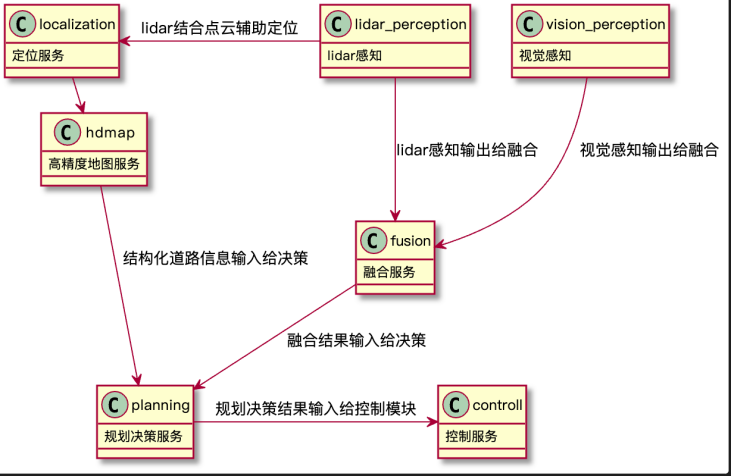
\includegraphics[width=0.65\textwidth]{3.1.png}
  \caption{自动驾驶单车内模块通信拓扑图}
  \label{fig:13}
\end{figure}
从图3.1可以分析出,模块之间通信主要是依次从上游原始数据传递到算法处理模块最终由下游的模块直接使用
并输出车辆的行为结果,此外还存在两个模块互相发送接收信息的模式。当系统内参与通信模块数量持续增加时,
通信的拓扑网络将变得复杂。针对自动驾驶系统中通信网络拓扑复杂的问题,采取基于话题的发布-订阅通信模式是
解决此问题的一个较好方法。

同时注意到一个模块发送的信息可以被多个模块接收,这代表同一份数据需要被传输到不同的模块中,结合第二章
论述的利用TCP/IP通信方式的特点,同一份数据需要被拷贝多次到不同的模块中,而单模块传输数据本身也需要
多次拷贝,如图3.2所示:
\begin{figure}[H]
  \centering
  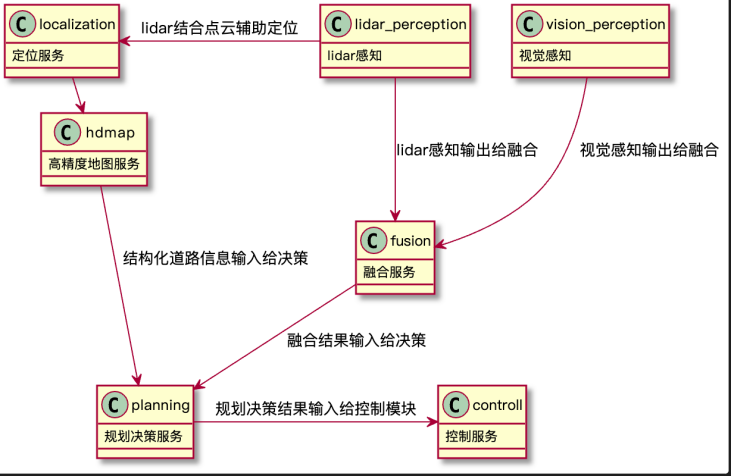
\includegraphics[width=0.65\textwidth]{3.1.png}
  \caption{自动驾驶单车内模块通信拓扑图}
  \label{fig:14}
\end{figure}
从图中可以看出当传输摄像机拍摄的图像等较大的数据时,数据的多次额外拷贝就会成为通信系统本身的性能瓶颈。
\subsubsection{单车与云端平台通信特点}
目前自动驾驶系统通信并不局限于车内各功能模块的通信,而是正迈向SOA架构风格。
即自动驾驶系统运行时需要的元数据、配置文件甚至路线的规划都逐渐从本地保存转变为与云端服务器进行数据的交互。
大部分自动驾驶系统是基于高精度地图来提供结构化道路信息供算法使用。高精度地图是一种精度更高,纬度更多,兼有动态数据和静态数据的
电子地图。高精度地图的生产的原则之一是反映实际道路的形态,当道路形态改变时,高精度地图将不再可靠。
在这种技术方案下,自动驾驶系统需要更新最新的高精度地图数据且频率并不低,所以自动驾驶系统需要频繁地去更新地图数据。
针对此问题,自动驾驶系统会在每次运行时都向云端的数据平台下载最新的地图数据,流程如图3.3所示:
\begin{figure}[htb]
  \centering
  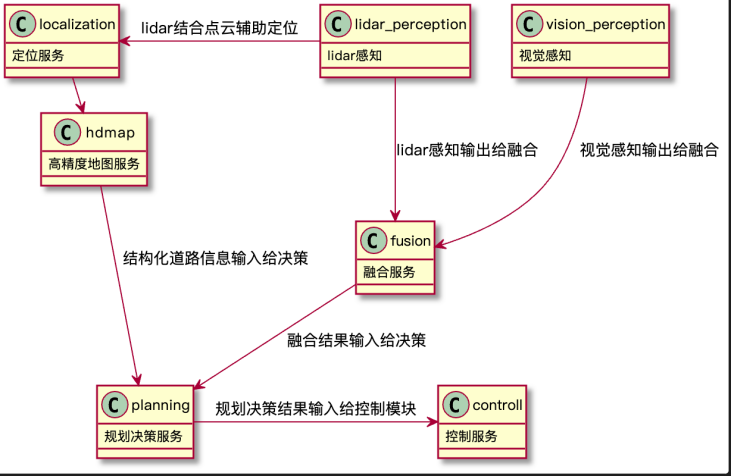
\includegraphics[width=0.65\textwidth]{3.1.png}
  \caption{自动驾驶单车内模块通信拓扑图}
  \label{fig:15}
\end{figure}
从此实际例子可以看出,自动驾驶系统通信已经不能局限于车内本地的通信,需要更多地考虑与云端或更多终端
进行通信的能力。更早地布局自动驾驶车辆与不同终端的通信能力可以实时地将数据同步到车内实现更好的自动驾驶
性能表现,同时未来也可以更快速地接入智能路网等应用。

综合本节阐述的自动驾驶单车内通信及单车与云端平台通信特点,可以得出自动驾驶系统对通信系统的要求是多样的。

在业务形态方面,传统的通信系统通常只提供单一的通信模式,限制了用户根据使用场景灵活调整通信模式的需求。而
自动驾驶要求通信系统具备多样化的通信模式,既要求通信系统具备进程间通信能力,还要求其具备网络通信能力,甚至
要求具备进程内通信能力。

\subsection{业务流程描述}
虽然自动驾驶运行时通信系统业务流程复杂,但从更抽象的角度来看,业务流程可大致分为如下四步:
\begin{enumerate}
  \item 申请通信:通信需求方提交通信目标及通信方式到通信系统等待系统返回申请结果。
  \item 通信校验:通信系统收到通信需求后,校验申请方的申请是否合法,若合法则进入通信匹配流程,否则直接终止流程。
  \item 通信匹配:通信系统寻找通信需求方的通信目标,若成功匹配到通信目标则进入到建立通信信道流程,否则进行等待通信目标出现直至超时终止流程。
  \item 建立通信信道:通信系统向通信双方通知通信信道建立,双方开始通信。
\end{enumerate}

图3.4是对建立通信业务流程的描述说明。
\begin{figure}[H]
  \centering
  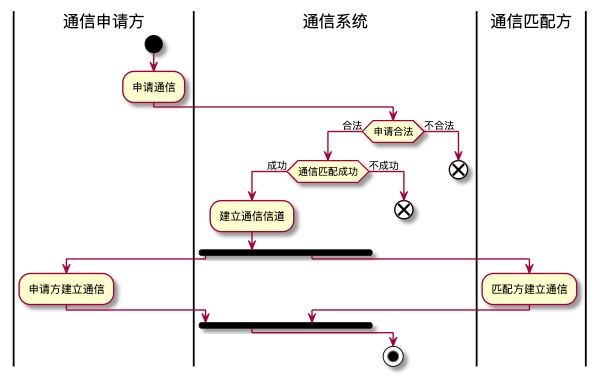
\includegraphics[width=0.7\textwidth]{3.4.jpg}
  \caption{建立通信业务流程图}
  \label{fig:16}
\end{figure}

\section{功能性需求}
根据上一节对自动驾驶系统通信的模式与特点的概述与分析,本文实现的自动驾驶运行时通信系统的功能需求
变得清晰,本节将导出本系统的功能性需求,并通过用例图对各个需求进行详细分析。

\subsection{通信单元管理}
注册通信单元功能是通信系统基本功能,自动驾驶系统的大部分通信功能都依托于数据发布者(publisher)发布数据
和数据订阅者(subscriber)订阅数据对通信单元实现准确、完备的管理不仅可以实现用户对管理通信单元多样的
需求,也是整个通信系统的基础。通信单元管理包括注册通信单元、删除通信单元、修改通信单元通信域和查询通信单元信息。

注册通信单元,分为注册数据发布者与注册数据订阅者,而数据发布者与数据订阅者又分为本机域通信和
全域通信。本机域通信规定通信单元只能在单机内通信;全域通信规定通信单元可以与任何通信单元进行通信。

删除通信单元,分为删除发布者与删除订阅者,其中删除订阅者分为立即删除与惰性删除两种模式。立即删除模式下,
订阅者会被直接删除,消息队列未接收的数据将被直接丢弃;惰性删除模式下,会首先将消息队列中未接收的数据保存再删除
订阅者。

修改通信单元通信域,分为修改发布者通信域与修改订阅者通信域,用户可以根据需要修改已经创建的发布者或订阅者
的通信域。

查询通信单元信息,分为查询发布者信息与查询订阅者信息,查询信息可以根据某一话题名称查询,也可以
查询所有存在的信息。同样地,用户可以根据实际需要查询本机内和全域内的通信单元信息。

通信单元管理用例图如图\ref{communication_unit_yongli}所示:
\begin{figure}[H]
  \centering
  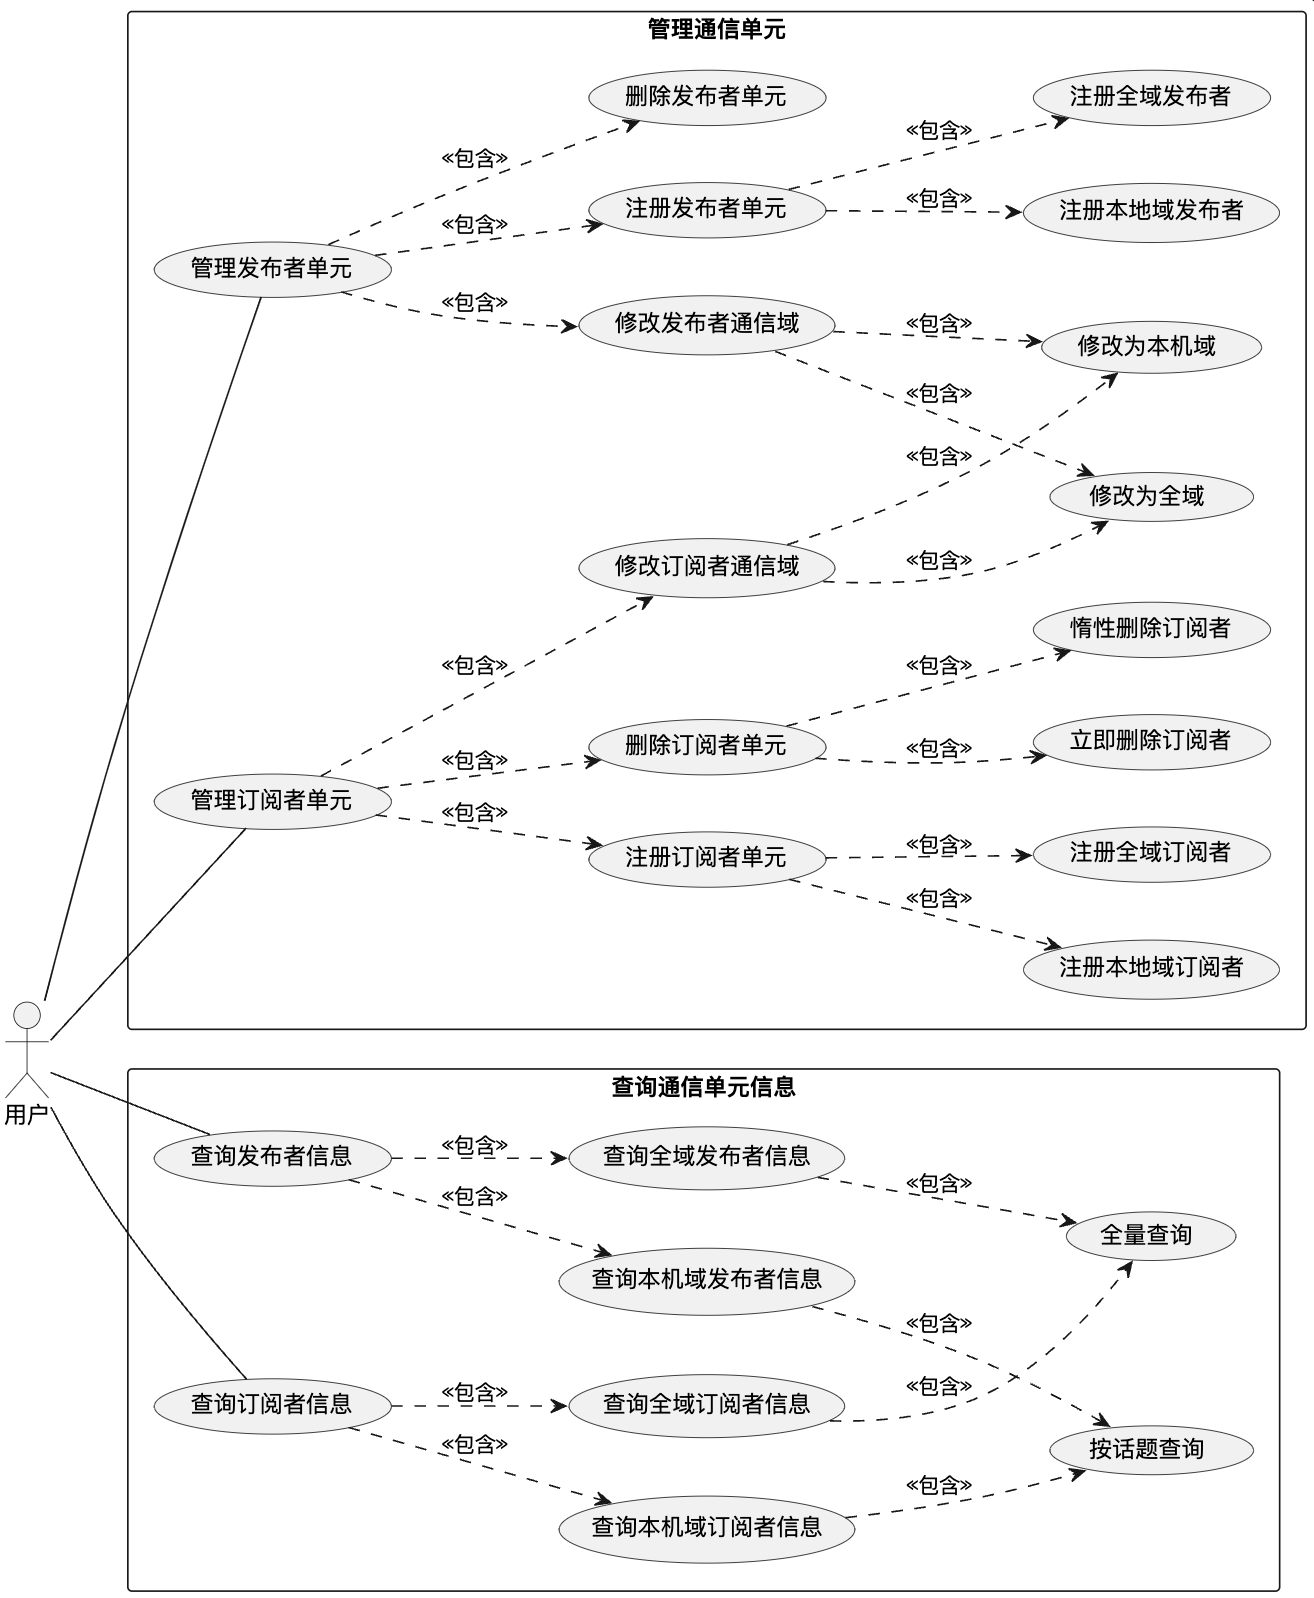
\includegraphics[width=0.75\textwidth]{communication_unit_yongli.png}
  \caption{通信单元管理用例图}
  \label{communication_unit_yongli}
\end{figure}

考虑到篇幅原因,本节仅以注册订阅者单元用例和删除订阅者单元用例为例说明,如表3.1和3.2所示:
\begin{table}[H]
  \centering\small
  \caption{注册订阅者单元用例说明}
  \label{tab:exampletable}
  \begin{tabular}{ll}
    \toprule
    \multicolumn{1}{l}{用例名称} & \multicolumn{1}{l}{注册订阅者单元}  \\
    \midrule
    行为角色 & 数据订阅者\\
    用例说明 & 注册订阅者单元,获得订阅数据能力;\\
    前置条件 & 发布者正确设置注册订阅者需要的参数;\\
    后置条件 & 注册订阅者单元成功,返回成功状态码;\\
    基本流   & \makecell[l]{1.设置订阅者订阅话题名称;\\2.设置订阅者发布数据的数据类型;\\3.设置订阅者订阅数据队列长度;\\4.设置订阅者通信域;\\5.提交参数到系统,注册成功,系统返回成功状态码;}\\
    异常流   & \makecell[l]{1a.数据订阅者未设置订阅话题名称,注册失败;\\2a.数据订阅者未设置数据类型,注册失败;\\3a.订阅者设置队列长度为非法大小,如负数等,注册失败;\\4a.订阅者未设置通信域,注册失败;}\\
    \bottomrule
  \end{tabular}
\end{table}
\begin{table}[H]
  \centering\small
  \caption{删除订阅者单元用例说明}
  \label{tab:exampletable}
  \begin{tabular}{ll}
    \toprule
    \multicolumn{1}{l}{用例名称} & \multicolumn{1}{l}{删除订阅者单元}  \\
    \midrule
    行为角色 & 数据订阅者\\
    用例说明 & 删除订阅者单元,停止订阅数据;\\
    前置条件 & 发布者正确设置删除发布者需要的参数;\\
    后置条件 & 删除订阅者单元成功,返回成功状态码;\\
    基本流   & \makecell[l]{1.设置删除模式;\\2.提交参数到系统,删除成功,系统返回成功状态码;}\\
    异常流   & \makecell[l]{1a.订阅者未设置删除模式,删除失败,系统返回失败状态码;}\\
    \bottomrule
  \end{tabular}
\end{table}
  
  
\subsection{服务管理}
在自动驾驶系统中,不仅仅需要给予发布-订阅模式的异步通信功能,还需要具备同步通信功能。当用户
注册了发布者和订阅者后,仅获得了最基本的异步消息收发能力,而服务的概念可以为用户提供更为高级的同步消息请求
能力,更契合自动驾驶系统SOA架构风格。在3.1节提到自动驾驶系统需要向云端数据平台请求高精度地图等数据,在这种情况下,
车端请求数据的动作的时间是不确定的,需要数据平台提供请求数据的服务,等待车端发起数据请求。

根据自动驾驶系统通信特点及用户的实际需要,服务管理包括创建服务、删除服务、修改服务通信域和查询服务信息。

创建服务,分为创建服务端与创建客户端,同通信单元的发布者和订阅者一样,服务端与客户端可以自由选择通信域。

删除服务,分为删除服务端与删除客户端,与通信单元不同的是,删除模式只有立即删除一种模式。

修改服务通信域,分为修改服务端通信域与修改客户端通信域,用户可以根据需要更改已经创建的服务客户端或服务端的通信域,
改变提供服务和请求服务的通信范围。

查询服务信息仅提供查询服务端相关信息,用户最关心的是系统中存在哪些服务端及其信息。查询可以通过服务端名称
进行查询,也可以进行全量查询,并且用户可根据需要确定在哪种通信域内进行查询。服务管理用例图如图\ref{service_yongli}所示。

\begin{figure}[H]
  \centering
  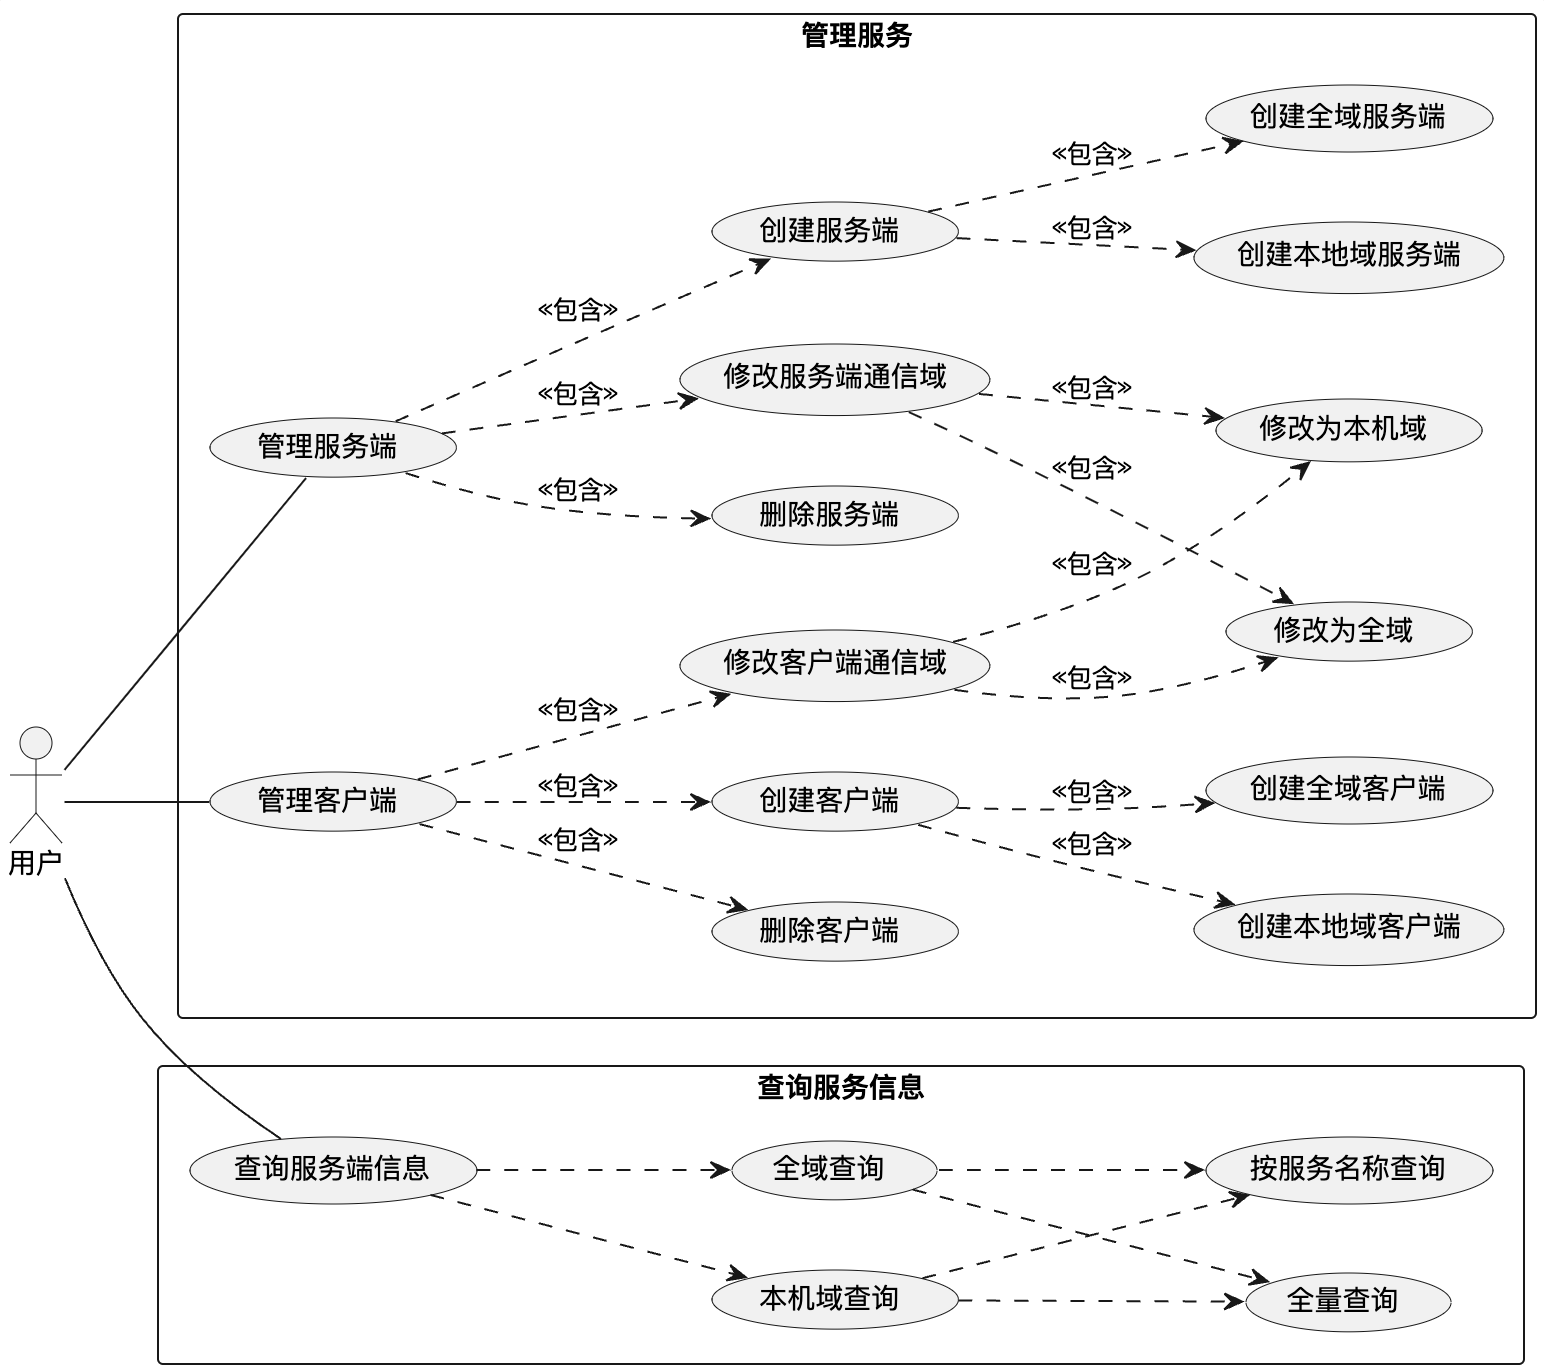
\includegraphics[width=0.85\textwidth]{service_yongli.png}
  \caption{服务管理用例图}
  \label{service_yongli}
\end{figure}

本节以创建服务端和查询服务信息用例为例进行说明,如图表3.3和3.4所示:
\begin{table}[H]
  \centering\small
  \caption{创建服务端用例说明}
  \label{tab:exampletable}
  \begin{tabular}{ll}
    \toprule
    \multicolumn{1}{l}{用例名称} & \multicolumn{1}{l}{创建服务端}  \\
    \midrule
    行为角色 & 服务提供者\\
    用例说明 & 创建服务,供服务使用者请求使用;\\
    前置条件 & 提供者正确设置相关参数;\\
    后置条件 & 创建服务成功,系统返回状态码;\\
    基本流   & \makecell[l]{1.设置服务名称;\\2.设置服务通信域;\\3.设置服务接收请求的数据类型;\\4.提交参数到系统,创建成功,系统返回成功状态码;}\\
    异常流   & \makecell[l]{1a.服务提供者未设置服务名称,注册失败;\\2a.服务提供者未设置服务通信域,注册失败;\\3a.服务提供者未设置接收请求的数据类型,注册失败;}\\
    \bottomrule
  \end{tabular}
\end{table}
\begin{table}[H]
  \centering\small
  \caption{查询服务信息用例说明}
  \label{tab:exampletable}
  \begin{tabular}{ll}
    \toprule
    \multicolumn{1}{l}{用例名称} & \multicolumn{1}{l}{查询服务信息}  \\
    \midrule
    行为角色 & 服务使用者\\
    用例说明 & 获取系统内服务端信息;\\
    前置条件 & 服务使用者正确设置相关参数;\\
    后置条件 & 删除发布者单元成功,返回成功状态码;\\
    基本流   & \makecell[l]{1.设置查询域;\\2.设置查询模式;}\\
    异常流   & \makecell[l]{1a.服务使用者未设置查询域,查询失败;\\2a.服务使用者未设置查询模式,查询失败;}\\
    \bottomrule
  \end{tabular}
\end{table}


\subsection{通信方式自适应选择}
通信方式是自动驾驶运行时通信系统核心功能之一,根据实际情况合理地选择通信方式是降低系统通信延迟、提高消息吞吐量的
关键。
为了避免ROS系统单一通信方式对通信性能的影响,并根据3.1节对自动驾驶通信特点的分析,本系统需要支持网络通信、进程间通信及进程内通信。
本系统在支持多通信方式的同时,需要根据通信双方是否处于同一台物理机和是否处于同一个进程自动选择网络通信、进程间通信或进程内通信方式
并协助通信双方按照通信方式建立通信链路。

通信方式自适应选择功能由通信系统内部的通信抽象层实现,通信方式自适应选择用例图如图\ref{adaptive_communication_yongli}所示。

\begin{figure}[H]
  \centering
  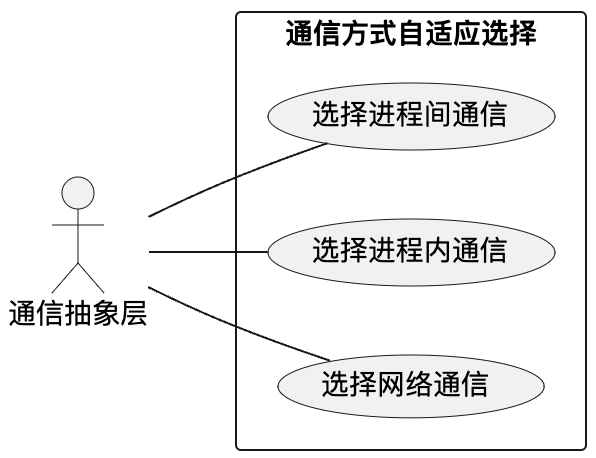
\includegraphics[width=0.55\textwidth]{adaptive_communication_yongli.png}
  \caption{通信方式自适应选择用例图}
  \label{adaptive_communication_yongli}
\end{figure}


% \subsection{进程间通信方式管理}
% 进程间通信方式决定了两个不同进程间发布者于订阅者通信的效率。用户希望进程间通信方式可以契合自动
% 驾驶系统通信的特点,可以根据用户实际需要来自由地选择进程间通信方式,而不是由系统本身强制用户使用规定的通信方式。
% 当用户需要在单车内传输数据量较大的数据如图片时,可以选用共享内存进行数据传输;当传输IMU(惯性测量单元等)等数据量较小
% 的数据时,可以选用网络进行数据传输。
% 因此,进程间通信方式管理是核心需求之一,进程间通信方式管理包括设置进程间通信方式与修改进程间通信方式。从通信方式的视角来看,
% 该用例的角色限定为订阅者。

% 修改进程间通信方式分为两种修改模式,立即修改与安全修改。立即修改修改模式下,系统将立即删除该通信节点的通信链路并
% 重新建立新的通信链路;安全修改模式下,系统将提前通知修改通信方式后受影响的通信单元,待剩余数据发送接收
% 完成后再重新建立通信链路。通信模式管理用例图如图3.7所示。

% 本节以设置进程间通信方式用例为例进行说明,如表3.5所示:
% \begin{table}[H]
%   \centering\small
%   \caption{设置进程间通信方式用例说明}
%   \label{tab:exampletable}
%   \begin{tabular}{ll}
%     \toprule
%     \multicolumn{1}{l}{用例名称} & \multicolumn{1}{l}{设置通信模式}  \\
%     \midrule
%     行为角色 & 订阅者\\
%     用例说明 & 设置通信单元的通信方式;\\
%     前置条件 & 正确填写相关参数;\\
%     后置条件 & 设置通信方式成功,返回成功状态码;\\
%     基本流   & \makecell[l]{1.设置进程间通信模式;\\2.设置进程间通信方式成功,系统返回注册成功;}\\
%     异常流   & \makecell[l]{1a.未正确设置进程间通信方式或进程间通信方式非法,设置失败;}\\
%     \bottomrule
%   \end{tabular}
% \end{table}
% \begin{figure}[H]
%   \centering
%   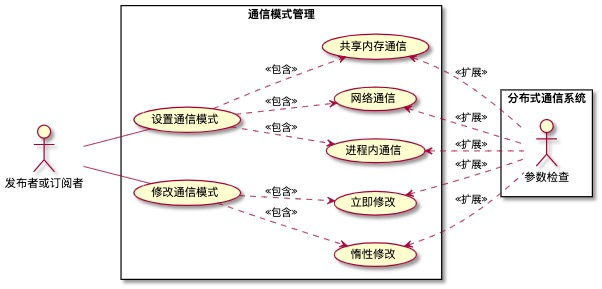
\includegraphics[width=0.8\textwidth]{3.7.png}
%   \caption{进程间通信方式管理用例图}
%   \label{fig:badge}
% \end{figure}

\subsection{调度策略管理}
自动驾驶对通信系统需求不仅是对通信功能的需求,还包含对任务调度方式的需求。同通信性能本身对整个通信
系统性能表现的影响程度,调度策略的选择一样重要。

在自动驾驶系统中,会存在多种传感器如摄像头、LiDAR(激光雷达)、IMU(惯性测量单元)等。自动驾驶对传感器发送
数据的频率有着较为严格的要求,通常会限定某个传感器在某个时间段内的平均频率为稳定在系统可接受范围内。针对此类
定频任务的实际需求,采用基于时间驱动的调度策略即每秒固定调度次数是较好的解决方法;传感器作为自动驾驶最上游的数据,
最终要经过处理供下游业务模块使用,而大多下游模块并不需要像传感器一样要求较为稳定的频率发送信息。此类业务模块
只需要关注何时收到了数据,并将数据运用到实际业务中,所以基于数据驱动的调度策适合该类任务的调度需求。
由此得出,系统需要提供调度策略管理功能给用户。调度策略管理提供给用户设置基于时间驱动调度策略的功能,基于数据驱动的
调度策略由通信系统内部自动设置,不需要用户手动设置。调度策略管理用例图如图\ref{schedul_yongli}所示。

\begin{figure}[H]
  \centering
  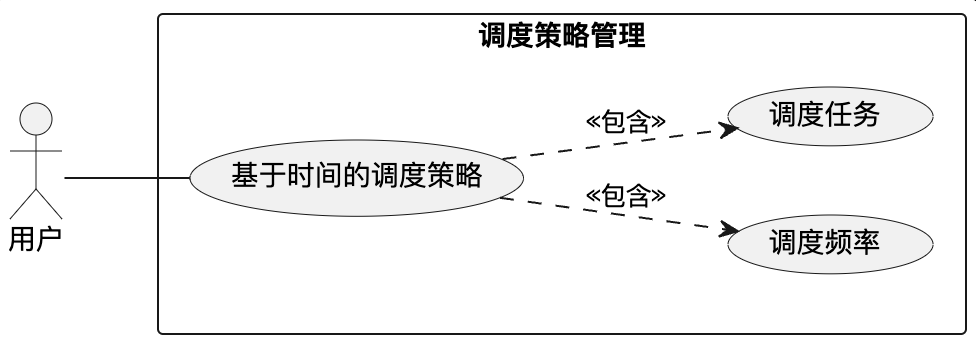
\includegraphics[width=0.75\textwidth]{schedul_yongli.png}
  \caption{调度策略管理用例图}
  \label{schedul_yongli}
\end{figure}

本节以设置基于时间驱动调度策略用例为例进行说明,如表3.5所示:
\begin{table}[H]
  \centering\small
  \caption{设置基于时间的调度策略用例说明}
  \label{tab:exampletable}
  \begin{tabular}{ll}
    \toprule
    \multicolumn{1}{l}{用例名称} & \multicolumn{1}{l}{设置基于时间的调度策略}  \\
    \midrule
    行为角色 & 发布者或订阅者\\
    用例说明 & 该用例实现对任务调度策略的设置;\\
    前置条件 & 已经注册通信单元;\\
    后置条件 & 设置调度策略成功,系统返回成功状态码\\
    基本流   & \makecell[l]{1.设置调度策略为基于时间;\\2.设置调度频率;\\3.设置成功,调度策略生效}\\
    异常流   & \makecell[l]{1a.未设置调度策略,设置失败;\\2a.未设置调度频率或调度频率为非法频率,设置失败;}\\
    \bottomrule
  \end{tabular}
\end{table}

\section{非功能性需求}
自动驾驶运行时通信系统在满足功能性需求的基础之上,还需要根据本系统实际应用场景满足非功能性需求。本系统应用在
算法模块数量庞大的自动驾驶系统中,非功能需求需要满足实时性、安全性、可靠性和可扩展性。

\subsection{实时性}
本系统的首要功能是向自动驾驶系统中各算法模块提供通信功能,
自动驾驶系统本身是对实时性要求非常高的系统,
本系统需要保证消息传输延迟保证在10ms之内并且不能出现较大波动。

\subsection{可扩展性}
本系统业务复杂,主要涉及不同方式的通信业务及复杂的用户接口设计,所以代码结构也同样复杂。
所以在实际的代码开发过程中需要尽可能将代码抽象为一个个独立的模块,模块之间通过预留的接口串联。
同时,本系统并没有使用较为流行的通信框架如DDS,模块化的设计思路可以快速地将更多的通信方式集成到系统中。

\subsection{鲁棒性}
本系统鲁棒性针对处于进程间通信模式下的发布者与订阅者和中心节点。当处于进程间通信模式下的任意发布者或订阅者由于程序崩溃导致异常退出后,其他发布者和订阅者
的通信不受影响;中心节点异常退出后应保证在5s内重新启动恢复正常。

\subsection{可靠性}
自动驾驶系统是个长时间运行的系统,连续运行5小时是对本系统的基本要求,通信系统需要具备长时间的可靠运行的能力。

\section{本章小结}
本章对自动驾驶运行时通信系统的应用场景进行深入分析,并从中导出功能性需求和非功能性需求。
一方面,功能性需求详细分析了本系统核心模块需要具备的功能;另一方面,实际应用的角度出发分析了本系统需要
保证的非功能性需求。








